%%%%%%%%%%%%%%%%%%%%%%%%%%%%%%%%%%%%%%%%%
% Beamer Presentation
% LaTeX Template
% Version 1.0 (10/11/12)
%
% This template has been downloaded from:
% http://www.LaTeXTemplates.com
%
% License:
% CC BY-NC-SA 3.0 (http://creativecommons.org/licenses/by-nc-sa/3.0/)
%
%%%%%%%%%%%%%%%%%%%%%%%%%%%%%%%%%%%%%%%%%

%----------------------------------------------------------------------------------------
%	PACKAGES AND THEMES
%----------------------------------------------------------------------------------------

\documentclass{beamer}

\mode<presentation> {

% The Beamer class comes with a number of default slide themes
% which change the colors and layouts of slides. Below this is a list
% of all the themes, uncomment each in turn to see what they look like.

%\usetheme{default}
%\usetheme{AnnArbor}
%\usetheme{Antibes}
%\usetheme{Bergen}
%\usetheme{Berkeley}
%\usetheme{Berlin}
%\usetheme{Boadilla}
\usetheme{CambridgeUS}
%\usetheme{Copenhagen}
%\usetheme{Darmstadt}
%\usetheme{Dresden}
%\usetheme{Frankfurt}
%\usetheme{Goettingen}
%\usetheme{Hannover}
%\usetheme{Ilmenau}
%\usetheme{JuanLesPins}
%\usetheme{Luebeck}
%\usetheme{Madrid}
%\usetheme{Malmoe}
%\usetheme{Marburg}
%\usetheme{Montpellier}
%\usetheme{PaloAlto}
%\usetheme{Pittsburgh}
%\usetheme{Rochester}
%\usetheme{Singapore}
%\usetheme{Szeged}
%\usetheme{Warsaw}

% As well as themes, the Beamer class has a number of color themes
% for any slide theme. Uncomment each of these in turn to see how it
% changes the colors of your current slide theme.

%\usecolortheme{albatross}
%\usecolortheme{beaver}
%\usecolortheme{beetle}
%\usecolortheme{crane}
%\usecolortheme{dolphin}
%\usecolortheme{dove}
%\usecolortheme{fly}
%\usecolortheme{lily}
%\usecolortheme{orchid}
%\usecolortheme{rose}
%\usecolortheme{seagull}
%\usecolortheme{seahorse}
%\usecolortheme{whale}
%\usecolortheme{wolverine}

%\setbeamertemplate{footline} % To remove the footer line in all slides uncomment this line
%\setbeamertemplate{footline}[page number] % To replace the footer line in all slides with a simple slide count uncomment this line

%\setbeamertemplate{navigation symbols}{} % To remove the navigation symbols from the bottom of all slides uncomment this line
}

\usepackage{structuralanalysis}
\usepackage{3dstructuralanalysis}

\usepackage{graphicx} % Allows including images
\usepackage{booktabs} % Allows the use of \toprule, \midrule and \bottomrule in tables


%----------------------------------------------------------------------------------------
%	TITLE PAGE
%----------------------------------------------------------------------------------------

\title[Structural Optimization]{Ottimizzazione Strutturale \\
	e \\
	Ottimizzazione Topologica } % The short title appears at the bottom of every slide, the full title is only on the title page

\author{Claudio Caccia} % Your name
\institute[Polimi] % Your institution as it will appear on the bottom of every slide, may be shorthand to save space
{
Progetto di Strutture Aerospaziali \\ % Your institution for the title page
\medskip
\textit{Politecnico di Milano} % Your email address
}
\date{\today} % Date, can be changed to a custom date

\begin{document}

\begin{frame}
\titlepage % Print the title page as the first slide
\end{frame}

\begin{frame}
\frametitle{Outline} % Table of contents slide, comment this block out to remove it
%\tableofcontents[hideallsubsections]
\tableofcontents
 % Throughout your presentation, if you choose to use \section{} and \subsection{} commands, these will automatically be printed on this slide as an overview of your presentation
\end{frame}

%----------------------------------------------------------------------------------------
%	PRESENTATION SLIDES
%----------------------------------------------------------------------------------------

%------------------------------------------------
\section{Descrizione del Problema} % Sections can be created in order to organize your presentation into discrete blocks, all sections and subsections are automatically printed in the table of contents as an overview of the talk
%------------------------------------------------

% \subsection{Modello Stutturale}
 % A subsection can be created just before a set of slides with a common theme to further break down your presentation into chunks

\begin{frame}
	\frametitle{Elementi dell'ottimizzazione strutturale:}
	\begin{itemize}
		\item modello strutturale
		\item modello di ottimizzazione
		\item algoritmo di ottimizzazione
	\end{itemize}
\end{frame}


\begin{frame}
	\frametitle{Modello di ottimizzazione}
	\begin{itemize}
		\item Modello strutturale:
			\begin{itemize}
				\item struttura reale $\Rightarrow$ modello
				\item funzione obiettivo e vincoli descritti come variabili del modello $\mathbf{x}$
			\end{itemize}
		\item Algoritmo di ottimizzazione:
			\begin{itemize}
				\item porta da soluzione iniziale $\mathbf{x_0}$ a $\mathbf{x_f}$
			\end{itemize}
		\item Modello di ottimizzazione:
			\begin{itemize}
				\item ponte tra struttura e algoritmo
				\item valuta f.o. e vincoli
				\item traduce le variabili strutturali in \textit{design variables}
			\end{itemize}
	\end{itemize}
	
\end{frame}


\begin{frame}
	\frametitle{Schema}
	Schema di ottimizzazione:
	\begin{figure}
		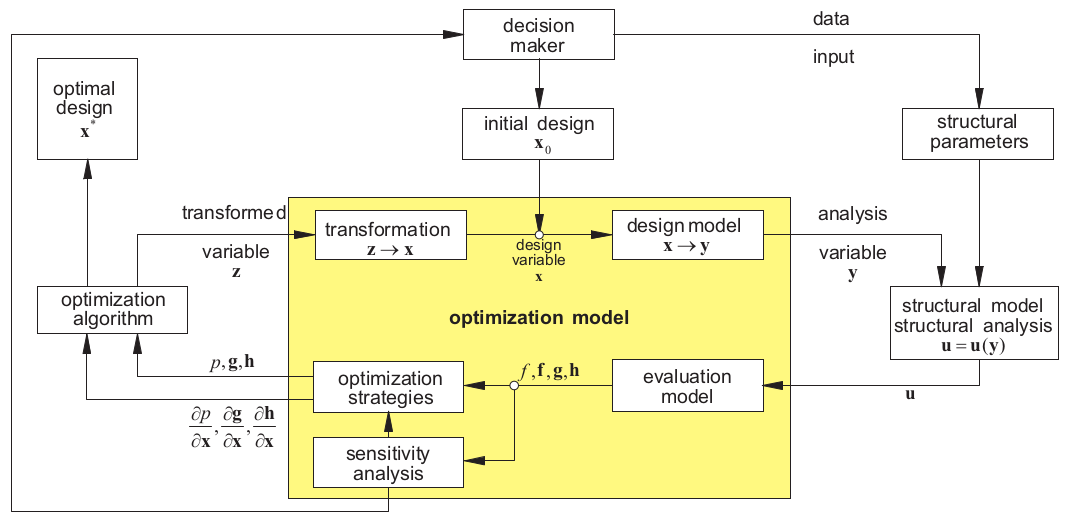
\includegraphics[width=0.8\linewidth]{./images/schema.png}
		\caption{Optimization schema \cite{eschenauer1997applied}}
		\label{fig:schema}
	\end{figure}
\end{frame}


%------------------------------------------------
\section{Definizione di un Modello di Ottimizzazione}
%------------------------------------------------




\begin{frame}
\frametitle{Formulazione}
 Forma generale \cite{vanderplaats1984numerical}:
	\begin{eqnarray}
	\underset{x}{\text{min}} & f(\mathbf{x}) & \mathbf{x} \in \mathbb{R}^n \\
	\text{subject to} & g_j(\mathbf{x}) \leq 0 & j=1,\ldots, m \\
	& h_k(\mathbf{x}) = 0 & k=1,\ldots, r \\
	&  \check{x_i} \leq x_i \leq \hat{x_i}  & i=1,\ldots, n
	\end{eqnarray}
\end{frame}


\begin{frame}
	\frametitle{Definizione dei termini}
	\begin{enumerate}
		\item Funzione obiettivo
		\item \textit{inequality constraints}: definiscono le regioni di validit\`{a} della f.o.
		\item \textit{equality constraints}: sono sempre attivi
		\item \textit{side constraints}: definiscono la regione di ricerca delle variabili
	\end{enumerate}
\end{frame}



%------------------------------------------------
\section{Categorie di modelli di Ottimizzazione}
%------------------------------------------------


\begin{frame}
	\frametitle{Categorie di Modelli}
	\begin{itemize}
		\item lineare, non-lineare \cite{vanderbei2014linear}
		\item continuo, discreto
		\item vincolato, non vincolato 
		\item convex optimization \cite{boyd2004convex}
		\item multi-objective \cite{desideri2010}
		\item modelli euristici vs. esatti
		\item metodi rilassati
		\item \ldots
	\end{itemize}
\end{frame}

%------------------------------------------------

\begin{frame}
	\frametitle{Note (1)}
	\begin{block}{Ottimizzazione multi-obiettivo}
		\begin{itemize}
			\item Frontiera di Pareto
			\item definizione a priori delle preferenze
			\begin{itemize}
				\item pb. di omogeneizzazione (costo?)
			\end{itemize}
			\item trasformazione di obiettivi in vincoli
		\end{itemize}
	\end{block}
\end{frame}

\begin{frame}
	\frametitle{Note (2)}
	
	\begin{block}{Convex optimization}
		In un certo senso pi\`{u} semplice. Strumenti molto potenti. Varie implementazioni software (ad es. \url{www.cvxopt.org})
	\end{block}

	\begin{block}{Rilassamento dei vincoli}
		Possibilit\`{a} di ridurre la complessit\`{a} del pb. modificando opportunamente i vincoli del problema.\\
		Varie tecniche, in particolare da \textit{binario} \textbf{[0,1]} a \textit{continuo}.
	\end{block}
\end{frame}


%------------------------------------------------
\section{Ottimizzazione strutturale: Classificazione}
%------------------------------------------------


\begin{frame}
	\frametitle{Ottimizzazione Strutturale}
	Classificazione dei modelli di O.S.\cite{christensen2008introduction}
	\begin{itemize}
		\item \textit{Sizing Optimization}
		\item \textit{Shape Optimization}
		\item \textit{Topological Optimization}
	\end{itemize}
\end{frame}



\begin{frame}
	\frametitle{Sizing Optimization}
	\begin{columns}[c] % The "c" option specifies centered vertical alignment while the "t" option is used for top vertical alignment
		
		\column{.35\textwidth} % Left column and width
		\textbf{Parametri}
		\begin{enumerate}
			\item Spessori
			\item Aree
			\item momenti d'inerzia
			\item \ldots
		\end{enumerate}
		
		\column{.6\textwidth} % Right column and width
		\begin{figure}
			\centering
			\begin{tikzpicture}
				\point{a}{0}{0};
				\point{b}{4}{0};
				\point{c}{4}{4};
				\beam{2}{a}{b};
				\beam{2}{b}{c};
				\support{1}{a}[-90];
				\support{1}{c}[180];
				\hinge{1}{a};
				\hinge{1}{c};
				\load{1}{b}[-210][1.2][-1.3];
				\notation{3}{a}{b}[$A_1$, E, $L_1$][.3][above right];
				\notation{3}{b}{c}[$A_2$, E, $L_2$][.5][right=2mm];
				\notation{4.5}{a}{b}[F][1][below right=2.2mm];
				\draw (4.5,0) arc (0:-30:0.5);
				\draw[line width=0.5pt] (4.1,0) -- (4.8,0);
				\node[] at (4.8,-0.2) {$\alpha$};
				\notation{5}{a}{b}[F][1][below right=4mm];;
			\end{tikzpicture}
			\caption[]{minimo peso con vincolo su sforzi}
			\label{fig:pc}
		\end{figure}
	\end{columns}
\end{frame}



\begin{frame}
	\frametitle{Shape Optimization (1)}
	Esempio:\\
	forma o contorno descritte in modo parametrico:
	\begin{figure}
		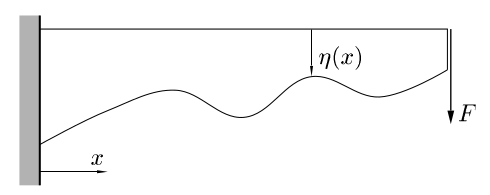
\includegraphics[width=0.7\linewidth]{./images/shape_ex.png}
		\caption{Shape Optimization}
		\label{fig:shape1}
	\end{figure}
	
\end{frame}


\begin{frame}
	\frametitle{Shape Optimization (2)}
	\begin{columns}[c] % The "c" option specifies centered vertical alignment while the "t" option is used for top vertical alignment
		
		\column{.35\textwidth} % Left column and width
		\textbf{Procedura}
		\begin{enumerate}
			\item def. parametri e limiti
			\item mesh
			\item risoluzione
			\item calcolo f.o.
			\item calcolo prossimo passo
		\end{enumerate}
		
		\column{.6\textwidth} % Right column and width
		\begin{figure}
			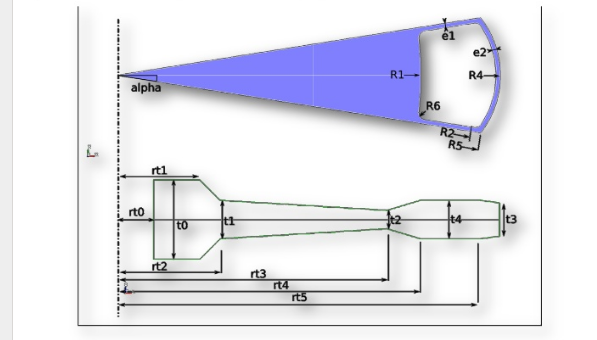
\includegraphics[width=0.9\linewidth]{./images/shape.png}
			\caption{shape opt.}
			\label{fig:shape}
		\end{figure}
	\end{columns}
\end{frame}


\begin{frame}
	\frametitle{Shape Optimization (3)}
	Metodi di \textbf{Design Improvement}
	\begin{itemize}
		\item Simplex
		\item Steepest Descent
		\item Conjugate Gradient
		\item Response Surface
		\item Line Search
		\item Brent
		\item Stochastic Search
		\item \ldots
		\item (DoE?)
	\end{itemize}
\end{frame}


\begin{frame}
	\frametitle{Ottimizzazione Topologica}
	Richiede il minor numero di informazioni iniziali:
	\begin{itemize}
		\item \textit{design space} (volume)
		\item vincoli
		\item carichi
	\end{itemize}
\end{frame}

\begin{frame}
	\frametitle{Esempio di O.T.(1)}
	Definizione del problema:
	\begin{tikzpicture}
	\point{a}{0}{0};
	\point{b}{7}{0};
	\point{c}{7}{2};
	\point{d}{0}{2};
	\beam{2}{a}{b};
	\beam{2}{b}{c};
	\beam{2}{c}{d};
	\beam{2}{d}{a};
	\support{2}{a}[-90];
	\support{2}{b}[0];
	\support{2}{d}[-90];
	\load{1}{d}[90][1.2][0];
	\end{tikzpicture}
	%\caption{O.T. - def. problema}
	\label{fig:schema_to}

\end{frame}


\begin{frame}
	\frametitle{Esempio di O.T. (2)}
	Soluzione:
	\begin{figure}
		\centering
		
\includegraphics[width=0.8\textwidth]{./images/beam_2d_reci_gsf_fine_100.png}
		%\caption{O.T. - soluzione}
		\label{fig:sol_to}
	\end{figure}
\end{frame}

%------------------------------------------------

%------------------------------------------------
\section{Ottimizzazione Topologica}
%------------------------------------------------

\begin{frame}
	\frametitle{Ottimizzazione Topologica [O.T.]}
	Consiste nello \textquotedblleft scavare \textquotedblright la struttura ottimale dal pieno:
	\begin{itemize}
		\item Definiti i vincoli
		\item Massimizzando la rigidezza del sistema (ma non solo)
		\item Data una percentuale prefissata di volume da mantenere 
	\end{itemize}
\end{frame}


\begin{frame}
	\frametitle{Nota}
	Nomenclatura (non ufficiale) in particolare per gusci: \\
	\begin{itemize}
		\item \textbf{Topology}: solid-void elements
		\item \textbf{Topometry}:sizing
		\item \textbf{Topography}: shape
	\end{itemize}
\end{frame}

\begin{frame}
	\frametitle{Topography optimization}
	\begin{figure}
		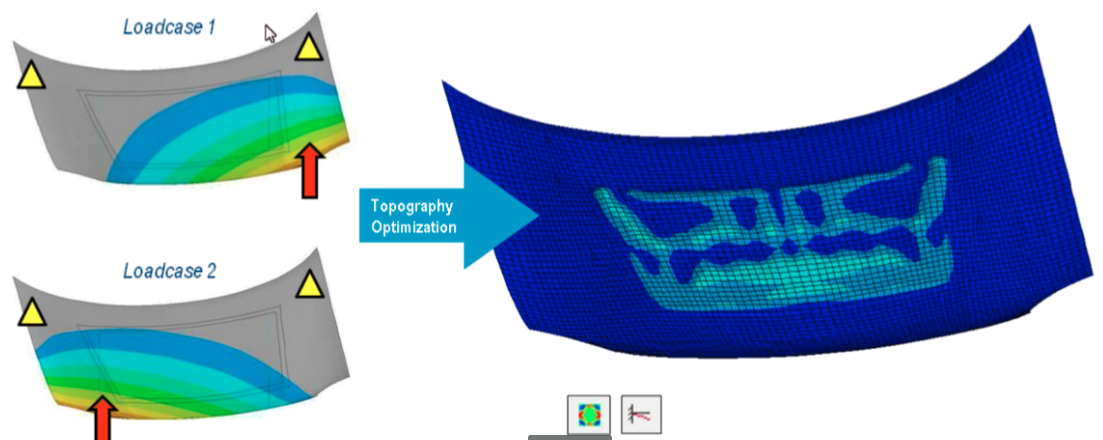
\includegraphics[width=0.9\linewidth]{./images/topography.png}
		\caption{topography opt.}
		\label{fig:topography}
	\end{figure}	
\end{frame}

\begin{frame}
	\frametitle{O.T. : Caratteristiche}
	Una volta definita una discretizzazione del dominio (\textit{mesh}) \\ il problema \`{e} intrinsecamente discreto (\textbf{binario}):
	\begin{itemize}
		\item un elemento partecipa \textbf{[1]}
		\item un elemento non partecipa \textbf{[0]}
	\end{itemize}
	alla soluzione finale
\end{frame}


\begin{frame}
	\frametitle{O.T. : Ricerca della soluzione}
	\begin{itemize}
		\item Il problema risulta intrinsecamente combinatorio
		\item Complessit\`{a} computazionale $\mathcal{O}(2^n)$
		\item moltissime soluzioni prive di significato
		\item non trattabile \textquotedblleft as is \textquotedblright per problemi anche semplici
	\end{itemize}
\end{frame}

\begin{frame}
	\frametitle{Definizione del Problema}
	Minimum compliance:
	\begin{eqnarray}
	\underset{x}{\text{min}} & f(\mathbf{x}) = \mathbf{q}^T \mathbf{f} & = \sum_{i=1}^{n}(x_i)^p \mathbf{q}_i^T \mathbf{K}_i \mathbf{q}_i \\
	\text{subject to} & g(\mathbf{x}) = & \frac{v_e}{v_0} \sum_{i=1}^{n}x_i - \bar{v} \leq 0 \\
	& \mathbf{K} \mathbf{q} = \mathbf{f} &  \\
	& 0 < \check{x_i} \leq x_i \leq 1  & i=1,\ldots, n
	\end{eqnarray}
			
	
\end{frame}

%------------------------------------------------
\section{OT: algoritmi}
%------------------------------------------------


\begin{frame}
	\frametitle{SIMP-like methods}
	\textbf{SIMP} Solid Isotropic Material with Penalization
	\begin{columns}[c] % The "c" option specifies centered vertical alignment while the "t" option is used for top vertical alignment
		
		\column{.35\textwidth} % Left column and width
		\begin{enumerate}
			\item homogeneization
			\item relaxed
			\item penalized
			\item continuus
		\end{enumerate}
		
		\column{.6\textwidth} % Right column and width
		\begin{figure}
			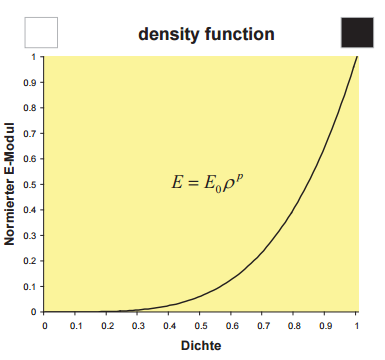
\includegraphics[width=0.7\linewidth]{./images/hom.png}
		\end{figure}
	\end{columns}		
\end{frame}




\begin{frame}
	\frametitle{SIMP}
	\begin{itemize}
		\item Largamente usato in codici commerciali
		\item produce valori intermedi delle variabili di progetto $x_i$
		\item eccessivi valori di penalizzazione rendono il pb malcondizionato o soggetto a minimi locali
		\item fase di \textit{postprocessing} per definire la geometria
		\begin{itemize}
			\item rispetta i vincoli?
			\item fattibile?
		\end{itemize}
	\end{itemize}
\end{frame}


%------------------------------------------------

\begin{frame}
	\frametitle{Sequential Approximate Optimization}
	S.A.O: \cite{haftka2012elements}
	\begin{itemize}
		\item 	Obiettivo: generare soluzione a predominanza di "pieni-vuoti"
		\item Approssimazione lineare locale del problema
		\item uso di \textit{intervening variables} per per linearizzare il problema
		\item Soluzione iterativa
	\end{itemize}
	
	\begin{eqnarray}
	\check{x_i} & \leftarrow & max(x_i - \delta, \rho_{min}) \\
	\hat{x_i} & \leftarrow & min(x_i + \delta, 1)
	\end{eqnarray}
	
\end{frame}


\begin{frame}
	\frametitle{Altri algoritmi}
	\begin{enumerate}
		\item \textbf{Optimality Criterion} (O.C.): \cite{bendsoe1989optimal}
		\begin{itemize}
			\item Espressione delle condizioni di KKT sulla Lagrangiana del problema
			\item Equivalente a S.A.O. sotto determinate ipotesi 
		\end{itemize}
		\item \textbf{Gray Scale Suppression} (G.S.S.): \cite{groenwold2009simple}
	\end{enumerate}
\end{frame}



%------------------------------------------------
\section{OT: esempi}
%------------------------------------------------








\begin{frame}
	\frametitle{Theorem}
	\begin{theorem}[Mass--energy equivalence]
		$E = mc^2$
	\end{theorem}
\end{frame}




\begin{frame}
	\frametitle{Table}
	\begin{table}
		\begin{tabular}{l l l}
			\toprule
			\textbf{Treatments} & \textbf{Response 1} & \textbf{Response 2}\\
			\midrule
			Treatment 1 & 0.0003262 & 0.562 \\
			Treatment 2 & 0.0015681 & 0.910 \\
			Treatment 3 & 0.0009271 & 0.296 \\
			\bottomrule
		\end{tabular}
		\caption{Table caption}
	\end{table}
\end{frame}



%------------------------------------------------

\begin{frame}[fragile] % Need to use the fragile option when verbatim is used in the slide
	\frametitle{Verbatim}
	\begin{example}[Theorem Slide Code]
		\begin{verbatim}
		\begin{frame}
		\frametitle{Theorem}
		\begin{theorem}[Mass--energy equivalence]
		$E = mc^2$
		\end{theorem}
		\end{frame}\end{verbatim}
	\end{example}
\end{frame}








%------------------------------------------------

\begin{frame}
	\frametitle{Figure}
	Uncomment the code on this slide to include your own image from the same directory as the template .TeX file.
	%\begin{figure}
	%\includegraphics[width=0.8\linewidth]{test}
	%\end{figure}
\end{frame}

%------------------------------------------------
\section{OT: implementazioni SW}
%------------------------------------------------

%------------------------------------------------

\begin{frame}
	\frametitle{Figure}
	Uncomment the code on this slide to include your own image from the same directory as the template .TeX file.
	%\begin{figure}
	%\includegraphics[width=0.8\linewidth]{test}
	%\end{figure}
\end{frame}



%------------------------------------------------
\section{Conclusioni}
%------------------------------------------------


%------------------------------------------------

\begin{frame}
	\frametitle{Figure}
	Uncomment the code on this slide to include your own image from the same directory as the template .TeX file.
	%\begin{figure}
	%\includegraphics[width=0.8\linewidth]{test}
	%\end{figure}
\end{frame}














%------------------------------------------------

\begin{frame}[fragile] % Need to use the fragile option when verbatim is used in the slide
\frametitle{Citation}
An example of the \verb|\cite| command to cite within the presentation:\\~

This statement requires citation \cite{p1}.
\end{frame}

%------------------------------------------------

\begin{frame}[allowframebreaks]
\frametitle{References}
\footnotesize{
			\bibliographystyle{plain}
			\bibliography{biblio}
		}
\end{frame}

%------------------------------------------------

\begin{frame}
\Huge{\centerline{The End}}
\end{frame}

%----------------------------------------------------------------------------------------





\end{document} 